\section{A family of compact predictors}
\label{sec:editorial-method}
Figure~\ref{fig:method-family} relates the two context and anchoring designs.
\textbf{Ours-1} denotes the original paired-context variant.
\textbf{Ours-2--5} identify the spatial decoder choices below; the identifiers
describe mechanisms and remain fixed across results.

\begin{figure}[!htb]
\centering
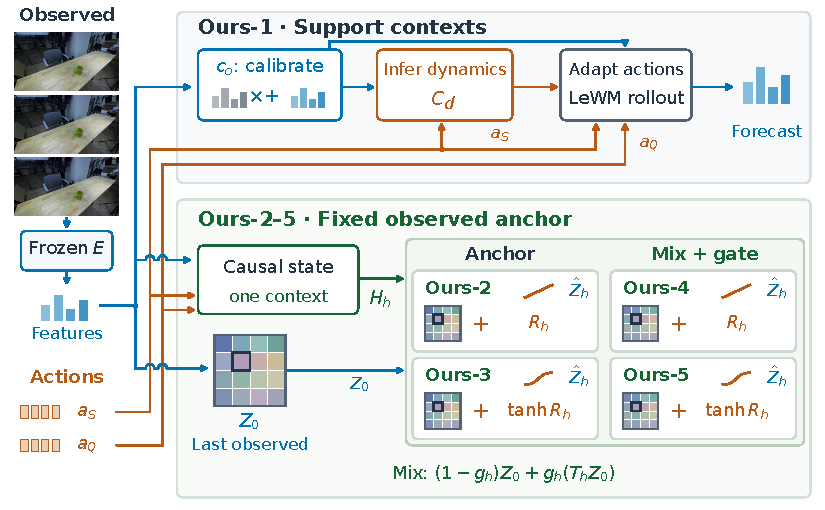
\includegraphics[width=\linewidth]{generated/editorial/method_family.pdf}
\caption[Method family overview.]{\textbf{Two ways to use observed evidence.} Ours-1 calibrates history with $c_o$, then infers $c_d$ from corrected transitions and past actions to condition LeWM. Ours-2--5 build a spatial state with past-only transition context and retain the last observed grid $Z_0$. Columns toggle gated row-stochastic feature mixing; rows toggle innovation bounding. Each cell specifies the future-feature forecast $\hat Z_h$. Recorded DROID images are unchanged (CC BY 4.0); latent colors are schematic. Shared interfaces do not imply shared weights, representations, or evaluation protocols. Detailed architectures and simulator-only planning appear in Appendices~\ref{app:spatial-development} and~\ref{app:original-context-study}.}
\label{fig:method-family}
\end{figure}


\subsection{Observation anchoring and action-conditioned mixing}
Let $Z_0\in\R^{16\times384}$ be the last observed DINOv2-small feature grid,
standardized using training-only channel statistics. A shared spatial encoder
maps each observed grid into 96-dimensional patch embeddings. The support
context uses only the observed transitions. A separate unidirectional GRU
encodes the chronological action prefix, and the reused temporal predictor
produces a horizon-specific patch state $H_h$. The observed support stays
fixed as the query horizon increases; no imagined image becomes new evidence.

Let $E_0$ denote the last observed spatial encoding before context modulation.
Queries from $H_h$ and keys from $E_0$ define a row-normalized mixing matrix:
\begin{equation}
 T_h=\operatorname{softmax}_{\rm row}\!\left(
 \frac{Q(H_h)K(E_0)^\top}{\sqrt{96}}+4I\right),\qquad
 g_h=\sigma(W_gH_h+b_g).
 \label{eq:editorial-mixing}
\end{equation}
The observed grid is the fixed source of the mixture. Ours-5 predicts
\begin{equation}
 \widehat Z_h=(1-g_h)\odot Z_0+
 g_h\odot(T_hZ_0)+\tanh R(H_h).
 \label{eq:editorial-forecast}
\end{equation}
Here $g_h$ is a per-patch gate, broadcast over channels; its bias initializes
at $-3$. The residual head $R$ uses normalization and an affine projection.
The mixture is over semantic feature patches and need not represent physical
pixel motion. Both the anchor and its encoding come from the last observation.

The factorial controls distinguish decoder choices:
\begin{equation}
\begin{array}{ll}
\text{Ours-2:}&Z_0+R(H_h),\\
\text{Ours-3:}&Z_0+\tanh R(H_h),\\
\text{Ours-4:}&(1-g_h)\odot Z_0+g_h\odot(T_hZ_0)+R(H_h).
\end{array}
\label{eq:editorial-variants}
\end{equation}
All use the same training data, feature coordinates and selection recipe.
The mixing package also contains its gate and identity bias and adds about
1.84\% active parameters. Its effect therefore concerns that complete package.

The row-normalized mixture gives a simple output-range property: for channel
$c$, each coordinate of its anchor component is a convex combination of
$Z_{0,:,c}$. Consequently Ours-5 satisfies
$|\widehat Z_{h,j,c}|\leq\max_k|Z_{0,k,c}|+1$ in standardized coordinates.
This is an architectural bound on values, not an accuracy or rollout-stability
guarantee. The component experiments test whether bounding improves accuracy.

\subsection{Intervention-paired context conditioning}
Ours-1 first infers observation context $c_o$ from past features and uses a
shared residual map to calibrate history and goal. It then infers dynamics
context $c_d$ from corrected transitions and executed actions, and conditions
the reused action embeddings. Training combines prediction and canonical
alignment losses with two consistency terms: the same physical trajectory
under different appearances should give consistent dynamics context, while
different trajectories with the same appearance should give consistent
observation context. Canonical renders and pairing identities are
training-only supervision. No simulator parameter enters inference.

Contexts and model weights remain fixed during each CEM search. All planning
controls share candidate counts, interaction budget and goal identities.
The detailed equations, paired losses and original architecture are retained
in Appendix~\ref{app:original-context-study}. The spatial models do not inherit
this two-context factorization or its paired simulator supervision.

\subsection{Relation to existing world models}
We build on pinned LeWM prediction and planning modules
\citep{maes2026lewm,maes2026stable}; compactness is an upstream property.
ContextWM and ICWM motivate conditioning on scene or interaction histories
\citep{wu2023contextwm,wang2026icwm}. MoVie and AdaJEPA study visual or online
adaptation \citep{yang2023movie,wang2026adajepa}; our evaluated predictors keep
their weights fixed at inference. ReDRAW and RLA-WM use residual modeling
\citep{lanier2025redraw,zhang2026rlawm}, so a residual head alone is not our
contribution. We investigate the fixed observed source of spatial mixing and
its controlled alternatives, alongside intervention-paired context learning.
DA-LeWM motivates separating predictive quality from planning-cost alignment
\citep{wang2026dalewm}. Our matched controls test these design choices; they
are not independent reproductions establishing state-of-the-art superiority.
